\documentclass[a4paper,11pt]{article}
%\usepackage{tabular}
\usepackage[dvipdfm]{graphicx}
\usepackage[dvipdfm]{color}
\usepackage{wrapfig}
\usepackage{amsmath, amssymb}
\usepackage{txfonts}
\usepackage{multirow}
\usepackage{subfigure}
\usepackage{ulem}
\usepackage{graphicx}
\usepackage{lscape}

\setlength{\textwidth}{150mm}  
\setlength{\textheight}{232mm}

\setlength{\oddsidemargin}{-2mm}
\setlength{\evensidemargin}{-2mm}
\setlength{\topmargin}{-15mm}
%%%%%%%%%%%%%%%%%%%%%%%%%%%%%%%%%%%%%%%%%%%%%%%%%%%%%%%%%%%%%%%
\begin{document}


\pagestyle{empty}

\begin{rightline}
{Jan-23-2014}
\end{rightline}
\noindent
\textbf{Plotting 1498 runs' entry time}\\

\noindent
1498 runs' entry time which were got from elog data are plotted.
This is different from event time.\\

\noindent
$\ast$ X axis tick-marks are located on Mondays.

\begin{figure}[htbp]
\begin{center}
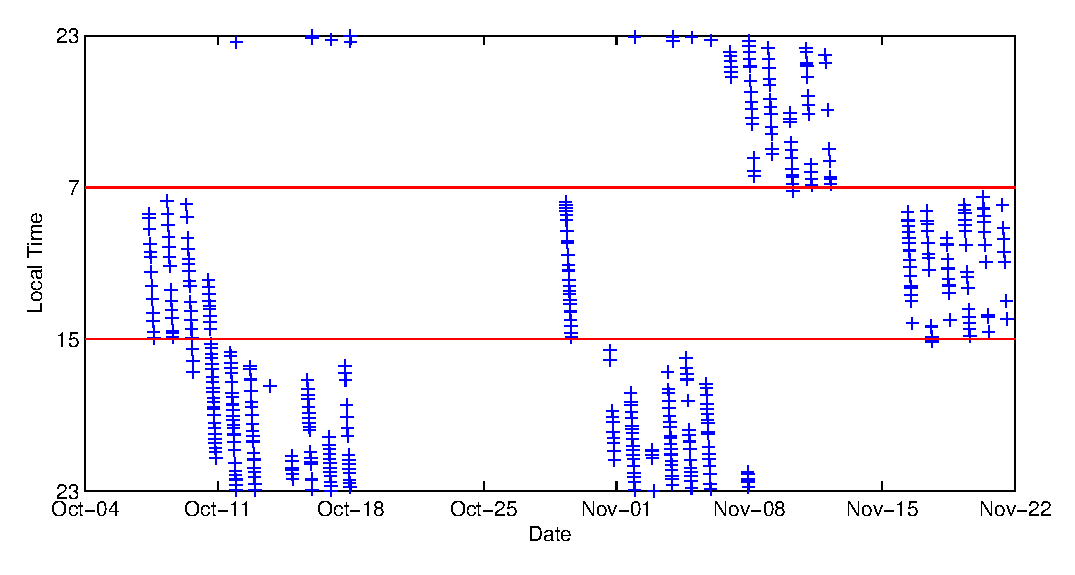
\includegraphics[width =11cm]{PlotTime2010.eps}
\caption{Entry Time Distribution - 2010}
\end{center}
\label{2010}
\end{figure}

\begin{figure}[htbp]
\begin{center}
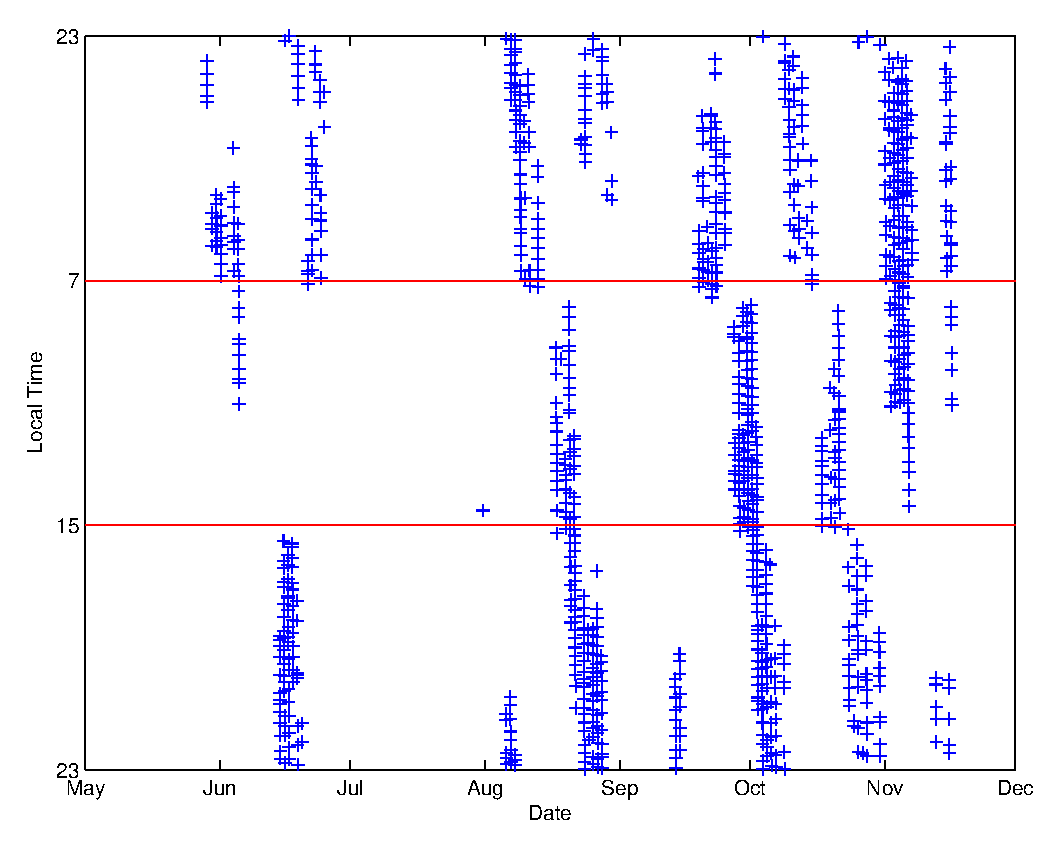
\includegraphics[width =11cm]{PlotTime2011.eps}
\caption{Entry Time Distribution - 2011}
\end{center}
\label{2011}
\end{figure}

\newpage

\begin{figure}[htbp]
\begin{minipage}{1.0\hsize}
\begin{center}
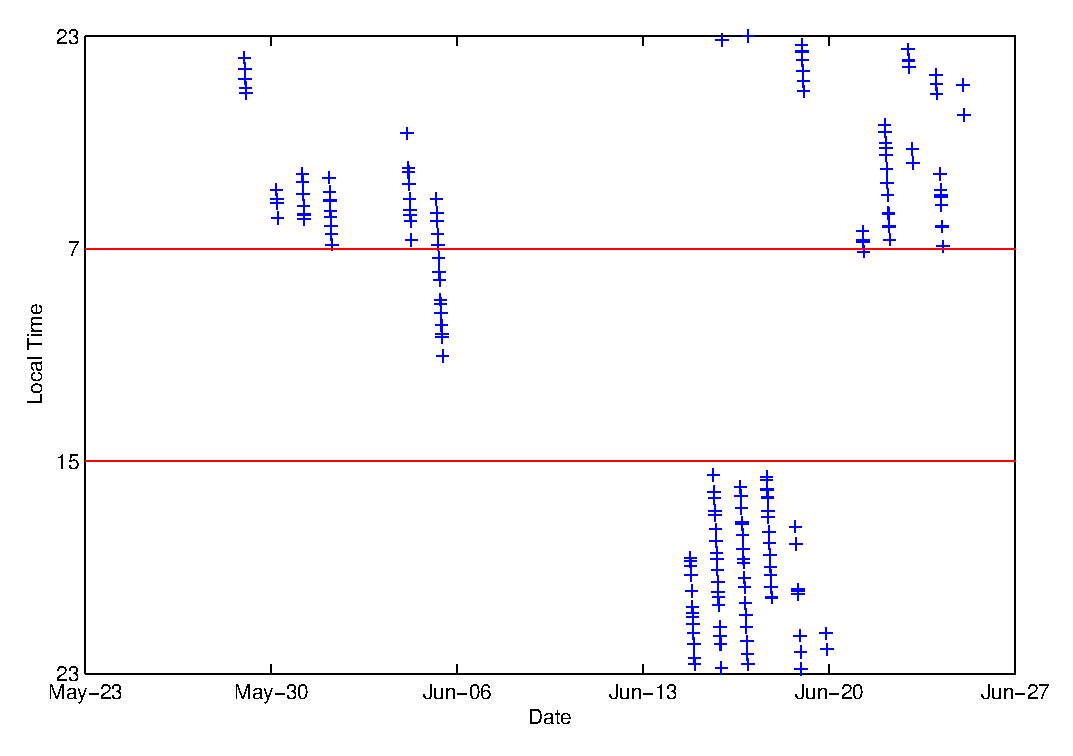
\includegraphics[width =8cm]{PlotTime2011_1.eps}
\\
\end{center}
\end{minipage}
\begin{minipage}{1.0\hsize}
\begin{center}
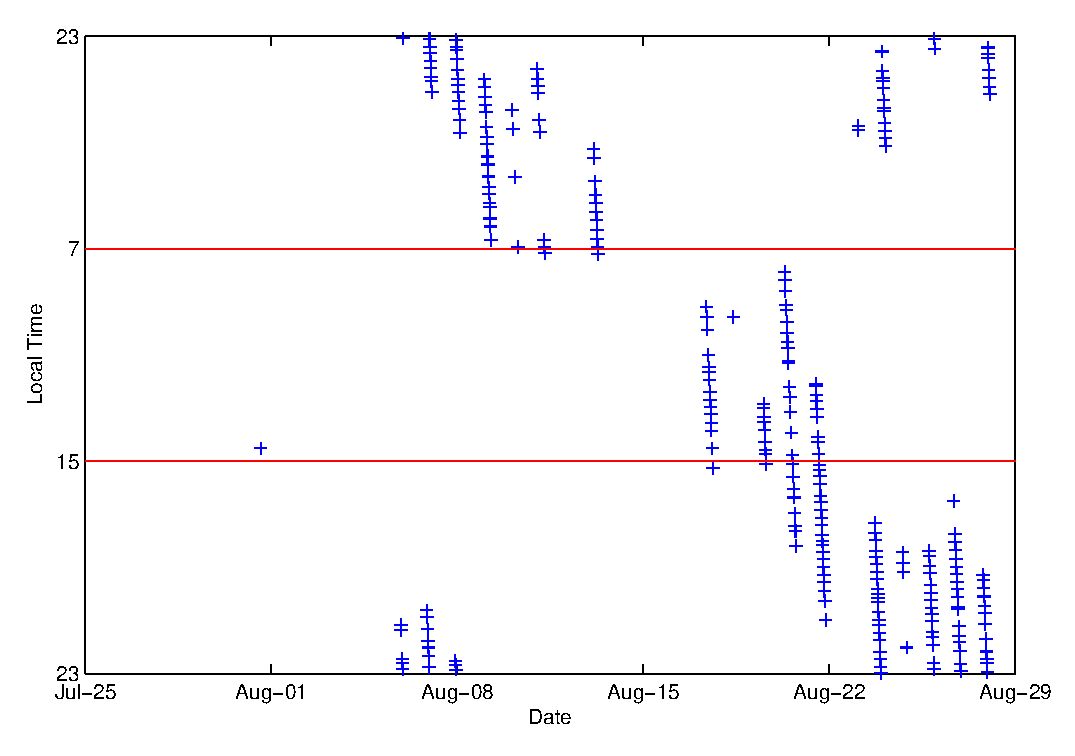
\includegraphics[width =8cm]{PlotTime2011_2.eps}
\\
\end{center}
\end{minipage}
\begin{minipage}{1.0\hsize}
\begin{center}
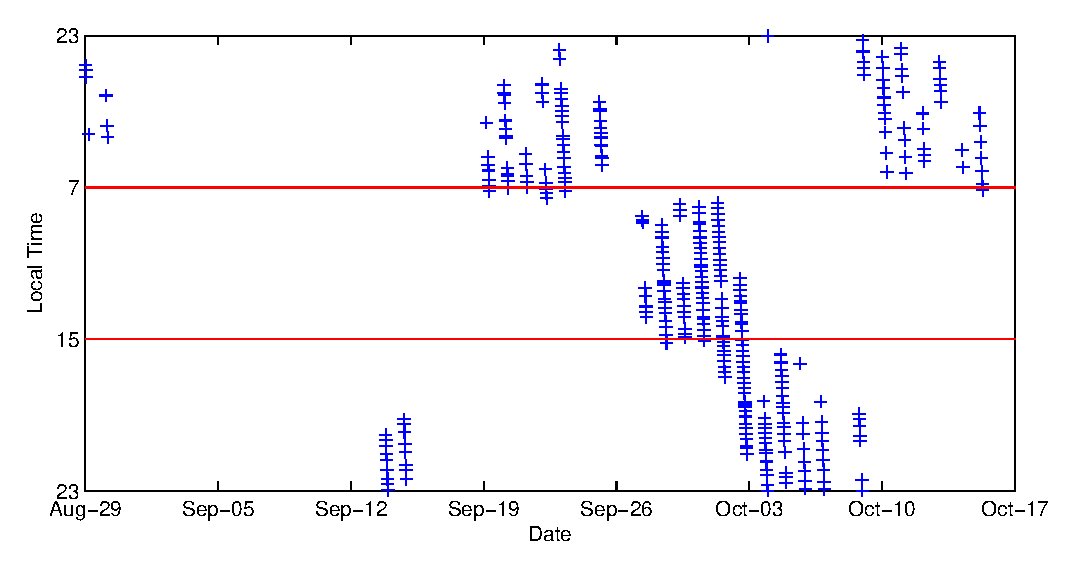
\includegraphics[width =9.6cm]{PlotTime2011_3.eps}
\\
\end{center}
\end{minipage}
\begin{minipage}{1.0\hsize}
\begin{center}
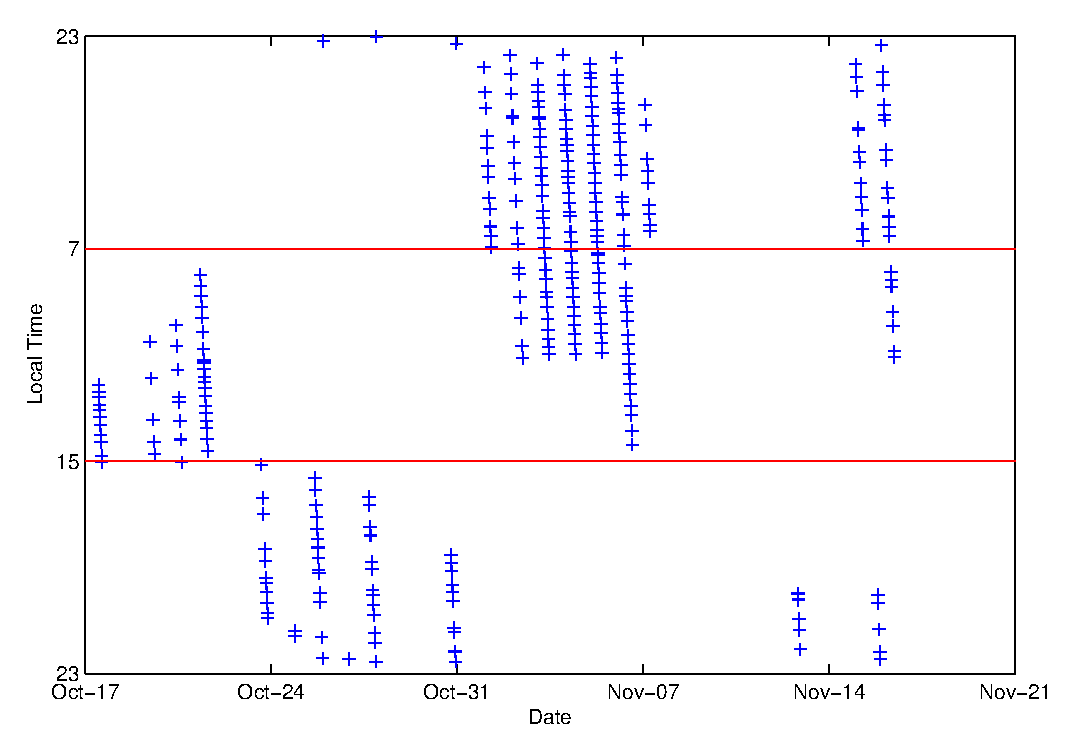
\includegraphics[width =8cm]{PlotTime2011_4.eps}
\\
\caption{Entry Time Distribution - 2011}
\end{center}
\end{minipage}
\end{figure}


 
\end{document}